\section{PDF: Structure, Complexity, Vulnerabilities}
\label{sec:pdf}

\subsection{The PDF Format}
\label{sec:pdfstructure}

\begin{figure}[t]
    \centering
    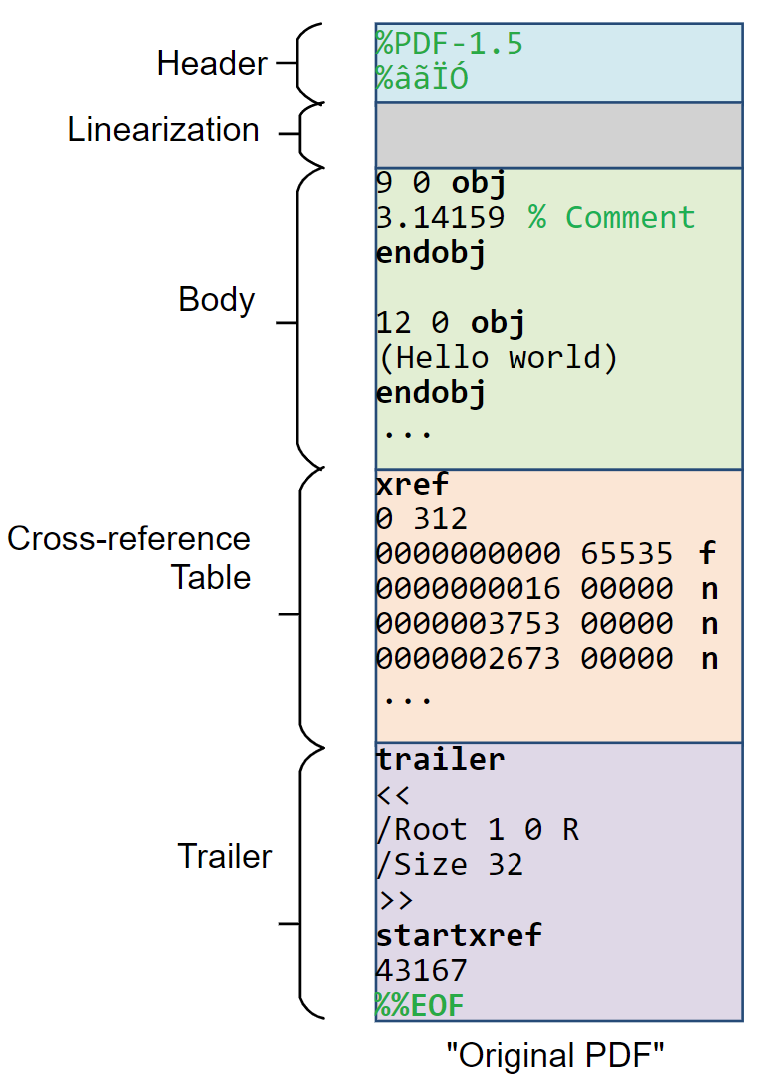
\includegraphics[width=0.65\linewidth]{figures/pdf-structure.png}
    \caption{The structure of a conventional PDF file: labeled sections with selections of representative grammar.}
    \label{fig:pdf-structure}
\end{figure}

PDF is a random-access file format that contains 8-bit binary data, line-based ASCII (7-bit)
text data (terminated with various end-of-line sequences), and a fixed format ASCII 
data format in different sections of a single file. The overall structure of a 
conventional PDF file without any incremental updates is shown in \cref{fig:pdf-structure} and 
described below, based on the official PDF ISO 32000 standard.
PDF 1.5 introduced more compact file structure capabilities known as cross-reference streams 
and object streams however, since this builds on the following concepts, this modern 
variation on the PDF file structure will be described later.

The PDF \emph{Header} section contains the file identification marker as an ASCII
text comment line \lstcd{\%PDF-} followed by the PDF version as single ASCII digits. 
An optional second comment line (starting with \lstcd{\%})
containing at least 4 bytes above 127 in value is recommended, to ensure 
that PDF files are not misidentified as purely 7-bit text files. 
All file offsets in PDF file are from the \lstcd{\%} sign in \lstcd{\%PDF-x.y}.  

The \emph{Linearization} section is an optional optimization section that enables what is commonly
known as ``fast web view''. This section must occur within the first 1024 bytes of a PDF and contains
data that enables a Linearized PDF aware parser to quickly display the opening page of a PDF
while the rest of a large PDF can download in the background.
Linearizatiom data is also invalidated by incremental updates (since an update might change objects
on the opening PDF page) and must therefore be checked and ignored.
%
Because not all PDF parsers support Linearization, it is a known form
of ``parser differential by design,'' where a \emph{parser
  differential} is a semantically meaningful difference in the result
of two parsers when run on the same document.
%
For the purposes of this paper, we will not consider Linearized PDF further.

The \emph{Body} section is where all indirect PDF objects are defined. Indirect PDF objects
are defined as those objects that have ``a unique object identifier by which other objects can
refer to it (for example, as an element of an array or as the value of a dictionary entry).''
Any PDF object may be defined indirectly: integers, real numbers, strings, arrays, dictionaries, 
streams, etc. Objects are defined by their object identifier (their object number and generation 
number pair) followed by the keyword \lstcd{obj}. 
The end of every object is defined by the keyword \lstcd{endobj}.
In \cref{fig:pdf-structure}, object 9 is a real number (in ASCII) followed by a comment
(introduced by \lstcd{\%}) and this is followed by object 12 which is a PDF literal string object
(enclosed in \lstcd{(} and \lstcd{)}).  
Every indirect object is reached by knowing the file offset to the start of the ASCII integer 
object number. This offset information for all indirect objects is stored in Cross-reference Tables.

The \emph{Cross-reference Table} section begins with the \lstcd{xref} keyword. For a PDF file
with no incremental updates, the next line will be a cross-reference sub-section text line comprising
two integers in ASCII (\lstcd{0 312} in this example). The first integer is an object identifier 
and in the case of an original PDF this must be 0. The second integer is the number of
objects in the cross-reference subsection.

There are two sets of
objects in every PDF document: the in-use list of PDF objects and a free list
of PDF objects. Object zero is always the start of the free list as it is not
otherwise a valid object number. Each incremental update may also move objects between these two sets.
In a conventional PDF, each entry for an object contains a fixed length 20-byte line of text.
The first 10 ASCII digits represent the byte offset to the object, followed by a single ASCII SPACE, 
followed by 5 ASCII digits representing an object generation number. This is then followed by
another single ASCII space and the keyword \lstcd{n} for in-use objects or \lstcd{f} for free objects.
Finally an end-of-line sequence is defined to ensure that the text line entry for each object has 
a 20-byte fixed length. A parsing subtlety is also that cross-reference sections are the only section 
in PDF where comments are expressly prohibited.

The \emph{Trailer} section is at the very end of every PDF file. 
It is defined as the end-of-file comment line \lstcd{\%\%EOF} immediately
preceded by the \lstcd{startxref} keyword followed by the file offset (in ASCII as a decimal) to 
the cross-reference table (i.e. the byte position of the \lstcd{xref} keyword 
from the the \lstcd{\%} of \lstcd{\%PDF-x.y}). Prior to this (but technically 
defined as being immediately \emph{after} the cross-reference table) is the trailer dictionary
identified by just the \lstcd{trailer} keyword, rather than the \lstcd{obj} and \lstcd{endobj}
keywords used in the PDF Body section.

\begin{figure}[t]
    \centering
    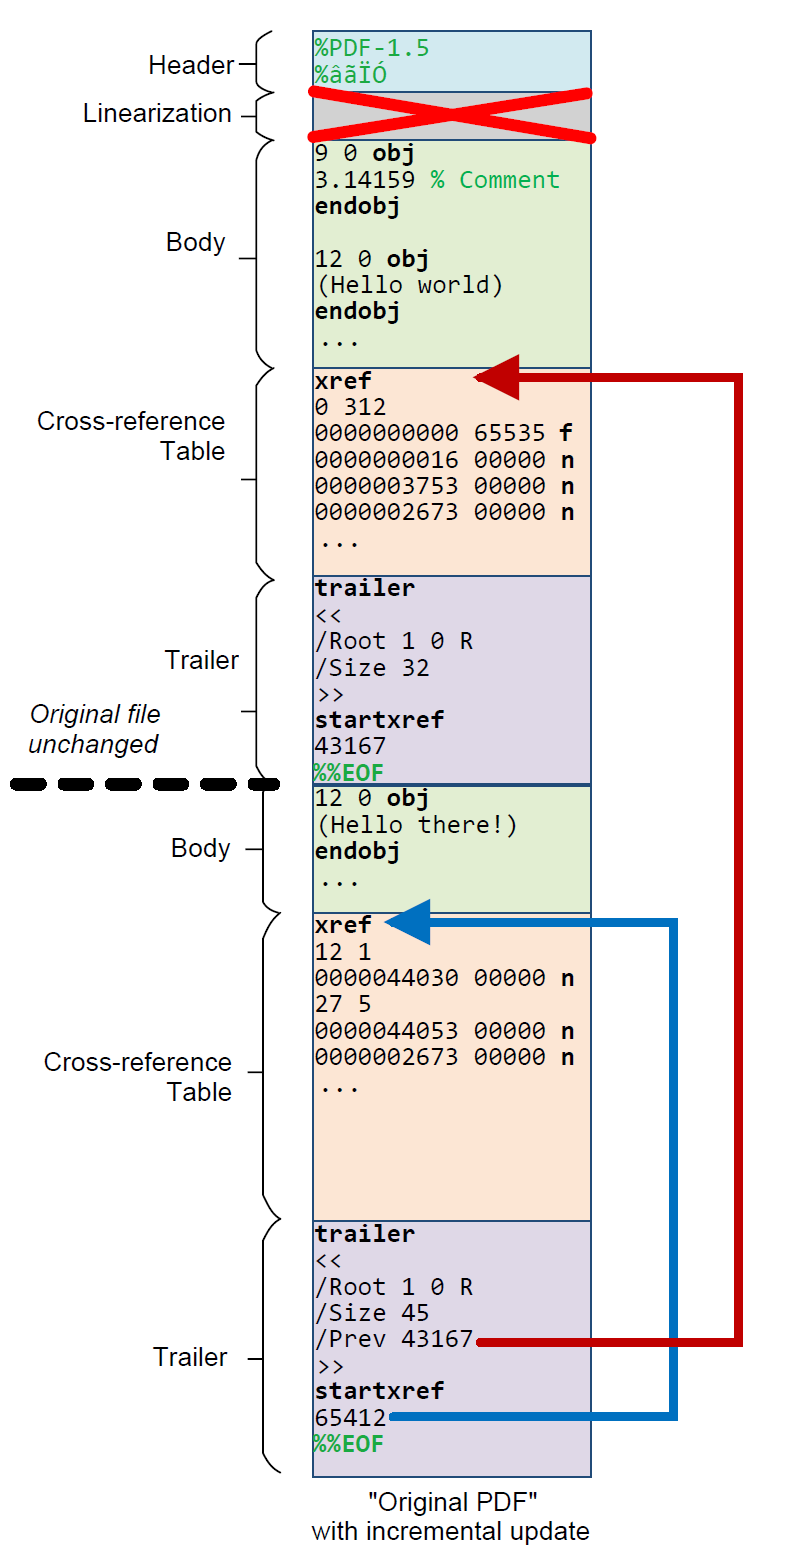
\includegraphics[width=0.65\linewidth]{figures/pdf-structure-incremental.png}
    \caption{Conventional PDF file structure with a single incremental update.}
    \label{fig:pdf-structure-incremental}
\end{figure}

As illustrated in \cref{fig:pdf-structure-incremental}, each incremental update will 
normally append a Body, Cross-reference Table, and Trailer sections
to a PDF file, with the entire original PDF remaining unchanged. The newly added incremental
update trailer dictionary must also contain information referencing the immediately 
previous cross-reference table by byte offset. The Body section of the incremental update 
will contain any new or redefined objects. If only fields in the trailer dictionary are updated then
a new Body section is not required. The cross-reference table for each incremental update
defines changes to objects made by that incremental update. This may include freeing
objects by adding them to the free list (the actual indirect PDF objects in
the PDF file are not actually deleted), and/or the addition of new objects. 

\begin{figure}[t]
    \centering
    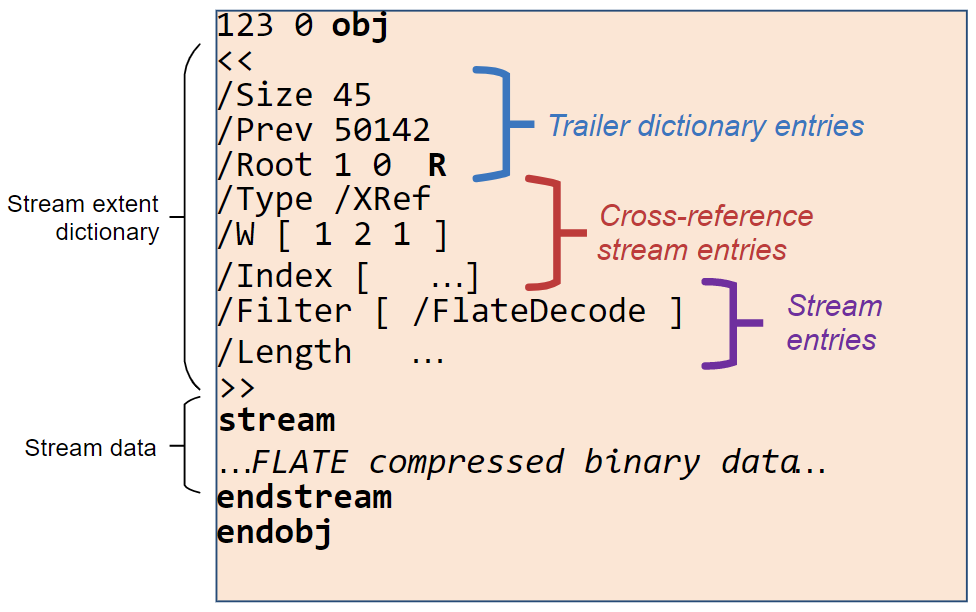
\includegraphics[width=0.65\linewidth]{figures/xrefstm.png}
    \caption{Example of a PDF 1.5 cross-reference stream.}
    \label{fig:XRefStm}
\end{figure}

As previously mentioned, PDF 1.5 introduced cross-reference streams and object streams as a means
to overcome physical file size limitations imposed by the 10-digit byte offset in the conventional
cross-reference tables.
Such files replace the Cross-Reference Table section (including the \lstcd{xref} keyword) 
with a PDF stream object containing binary data, as shown in \cref{fig:XRefStm}. 
Like all streams in PDF, cross-reference streams may also be compressed with algorithms such as FLATE 
to further reduce file size. If a cross-reference stream is used, then the trailer dictionary is also no
longer used. Instead the context-defining key/value pairs of the trailer are added to the stream 
extent dictionary of the cross-reference stream.

\begin{figure}[t]
    \centering
    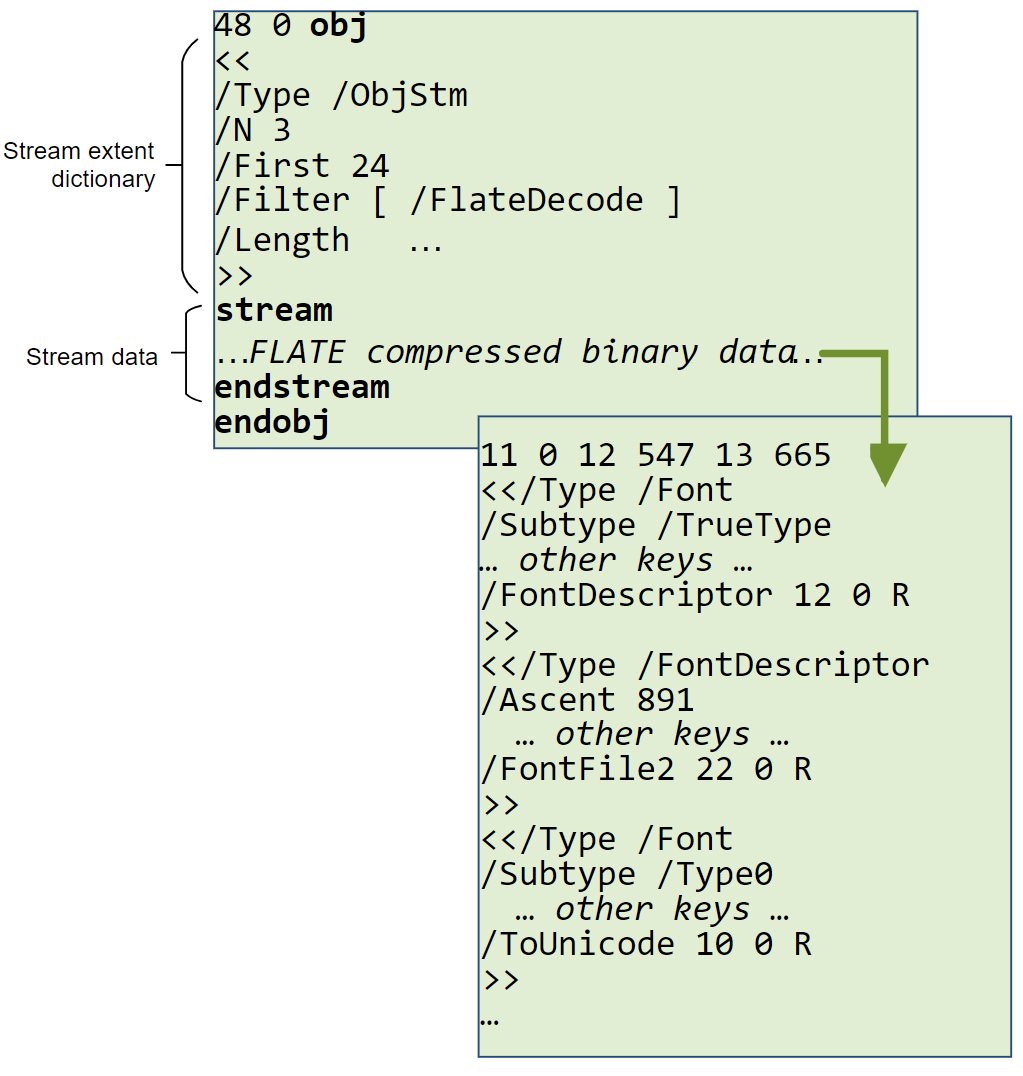
\includegraphics[width=0.65\linewidth]{figures/ObjStm.png}
    \caption{Example of a PDF 1.5 object stream and its uncompressed content.}
    \label{fig:ObjStm}
\end{figure}

PDF 1.5 enabled further optimization via object streams (\cref{fig:ObjStm}).
%
Practical large PDF's will typically contain many indirect objects;
%
thus the repeated use of the object identifier pair with \lstcd{obj}
and \lstcd{endobj} keywords can consume a significant amount of space.
%
Object streams are compressible text streams ``\ldots in which a
sequence of indirect objects may be stored, as an alternative to their
being stored at the outermost PDF file level.''
%
In place of keywords and object-identifier pairs, object streams use a
single object number and a byte offset within the object stream.
%
This ASCII text data can be aggressively reduced using algorithms for
stream compression.
%
If object streams are used, then cross-reference streams must also be
used.
%
However cross-reference streams may also be used by themselves with
the conventional Body section.

As noted above, because both cross-reference streams and object
streams are standard PDF streams, they can benefit from stream
compression. However this also means that parsers are susceptible to
attacks represented by compressed files of a tractable size whose
uncompressed data is much larger and intractable to process (i.e.,
``ZIP bombs''), cycles in object references, and handling of semantic
errors (invalid stream extent dictionaries) during pre-DOM processing.

PDF structure is further complicated in the case of
``hybrid-reference'' files, where both conventional cross-reference
tables and cross-reference streams co-exist to support parsers unaware
of PDF 1.5.
%
Such files are not addressed in this work.

The number and types of incremental updates that can be added to a
file are unlimited.
%
Later updates may ``undo'' changes from any previous incremental
updates by restoring (changing back to in-use) objects previously
feed.
%
PDF objects need not be numbered sequentially, with skipped object
numbers assumed to be on the free list (although the standard does not
state this explicitly).

In effect, incremental updates form a timeline of all changes made to
a PDF, with parsing starting at the end of the file with the most
recent change back to the original document at the to of the file.

\subsection{Root Causes of PDF Complexity}
\label{sec:rootcause}

Most data formats can be described by much simpler mechanisms;
most language processors (e.g., a Python parser) can be described and parsed by
textbook methods (e.g., \emph{lex} and \emph{yacc} are sufficient for
most language processors);
so what makes PDF processing so much more complex?

As described above, PDF uses random access to byte offsets to then parse lines of text,
which may then switch to binary data or fixed-length record parsing. 
In some, but not all, cases the end of an object can be known apriori, but in the most common case 
of conventional cross-reference tables, only forward parsing can determine the end of an object. 
This gives rise to a phenomena we call \emph{cavities} where not every byte in a PDF file is parsed.
Such cavities can be used to hold data in an alternate format giving rise to polyglots, or potentially
to hold shellcode that might be na\"ively loaded into memory and further exploited 
in vulnerable parsers.
In addition, various descriptions in the PDF standard require ``parsing backwards'' which is 
an unnatural programming language idiom. Furthermore, some explicit pre-DOM requirements
in the PDF standard
refer to bytes \emph{before} a given byte offset and that parsers are highly unlikely to check. 
Our investigations reveal that these requirements are effectively ``writer requirements'' (unparsers) to
support better file reconstruction and recovery in the event of later data corruption. 
However if these requirements are never checked or enforced then it is possible to use them as attack
vectors.  
The PDF specification also requires multiple
sublanguages and computation (such as stream decompression).

If a PDF file accidentally or maliciously fails to adhere to this set of complex PDF file structure
rules, or an implementation has bugs, PDF parsers will typically silently attempt to recover
by reconstructing the cross-reference table information. 
This is not defined by the PDF file format standard so 
ad-hoc algorithms are used. Typical reconstruction algorithms parse from the start of a PDF 
file, searching for indirect PDF objects (\lstcd{x y obj ... endobj}) at the start of lines. This can clearly result
in ambiguous reconstruction of a PDF DOM and is highly likely to lead to parser differentials.

The PDF DOM created by a set of indirect PDF objects forms a directed graph. 
Each PDF object is a vertex and indirect references between objects form the directed edges. It is 
specifically \emph{not} acyclic as PDF formally defines concepts such as parent references to 
pages and other objects. This is different to most XML-based file formats because XML naturally 
forces hierarchical relationships via nesting of tags.

The PDF standard defines very few explicit data integrity relationships for pre-DOM parsing. 
Our work has been to critically review the under-appreciated and under-studied pre-DOM PDF
file structure using formal methods to highlight data integrity relationships that can 
ensure the PDF Trust Chain is robust prior to DOM processing.

% ------------------------------------------------------------------------------
\subsection{Vulnerabilities}
\label{sec:vulnerabilities}

% As will become even more apparent, there is a significant amount of
% parsing and computation that needs to be done \emph{pre-DOM}.

The majority of prior work researching PDF vulnerabilities start with a pre-existing PDF DOM,
ignoring pre-DOM parsing and processing~\cite{smutzMaliciousPDFDetection2012,liuDetectingMaliciousJavascript2014,iwamotoStudyMaliciousPDF2016}. 
This work typically looks for obfuscated PDF objects such as
JavaScript streams or strings, action objects, URL strings, or file attachment objects that 
can lurk in various places throughout the PDF DOM. Machine-learning approaches so far have not  
used feature vectors based on the contextual information in PDF pre-DOM file structure~\cite{andrewmangleAnalysisMachineLearning2021,manharmohammedHAPSSAHolisticApproach2021}. 
Prior work in privacy has identified that incremental updates obviously pose a risk for complete
redaction and data scrubbing workflows if not processed correctly~\cite{adhataraoHowArePDF2021,y.fengSystematicMethodPDF2018}.
Given our recent points about the \emph{PDF Trust Chain}~\cref{sec:trust-chain}, it should not 
surprise us that some PDF attack vectors involve aspects of breaking the \emph{DOM} abstraction.
I.e., the root cause occurs pre-DOM.

\emph{Supply Chain attacks} generalize \emph{Shadow
  Attacks}~\cite{mainkaShadowAttacksHiding2021}, wherein an attacker
infiltrates a workflow and manipulates a document maliciously,
potentially creating a document that is entirely valid.
%
Only later in the workflow, possibly after a digital signature is
applied or an official approval step, the malicious data is
activated.
%
In the case of digitally-signed documents, this severely undermines
confidence and trust in digital signature technology.

\todo{we are using both 'parser differential' and ``ambiguous'': use one. 
They are different but related: In the intro we define ambiguities as ONE cause of parser 
differentials. In the PDF section I already wrote about "differential by design" caused 
by Linearized PDF. Is a parser differential necessarily something that a human can see? 
I would assert it is as you define below - so an ambiguity can also lead to a vuln which 
may not be noticeable (secret leak, etc). }

\emph{Parser Differentials} are a real threat as attackers leverage
differences in output to present different information to different
individuals, where the individual might be a human or a
machine. Parser differentials arise due to a combination of parser
weaknesses, parser permissiveness, ambiguities, and unexpected
input. In the case of PDF pre-DOM file structure, we have been able to
easily demonstrate parser differentials \todob{put small example here
  or ...? Could reference this PoC:
  https://github.com/pdf-association/safedocs/tree/main/Miscellaneous%20Targeted%20Test%20PDFs#dual-startxrefpdf
  or the vuln we discovered that is quoted back in the intro }

\emph{Polyglots} are a potential threat in any system or workflow
which relies on different parsers at different stages. If a firewall
product determines a file to be of file type \emph{X} and then only
scans for vulnerabilities relevant to file type \emph{X}, but later
software decides the same file is file type \emph{Y}, an organization
is then vulnerable.  Polyglots arise from the creative use of
cavities, permissive implementations, and other blind spots in a file
format specification where arbitrary data can be placed that does
impact processing (e.g. in comments or strings, in freed or
unreferenced objects, etc.).

\emph{Denial of Service (DoS)} is of increasing concern to PDF users,
with many PDF services and products utilizing cloud-based processing.
%
In cases such as large-scale automated invoice processing, DoS attacks
can also incur additional expenses as well as inconvenience for an
organization because exceptions may need to be handled by human
operators.

% many errors exist:
Due to the complexity and subtleties of the PDF standard described
above, extant data exhibits many errors in cross-reference tables and
related pre-DOM context information.
%
To date, there has not been a comprehensive analysis of PDF file
structure faults in extant data caused by defects in PDF writers, due
in part to a lack of tooling that comprehensively reports all
variations from the standard.
%
However, analysis of open-source PDF parser code bases does highlight
tools with varying degrees of lightweight reporting, however all
exhibit permissive features related to pre-DOM processing:
%
\begin{itemize}
    \item deviation from the required 20-byte fixed cross-reference table entry, with support for
    19- and 21-byte variations due to additional white space or incorrect line endings;
    \item errors in byte offsets to indirect PDF objects and objects in object streams;
    \item errors with \lstcd{startxref} byte offsets;
    \item incorrect trailer dictionary data (such as \lstcd{Size}), leading to implementation-dependent decisions;  
    \item terminating pre-DOM processing prematurely (i.e. not processing all incremental updates and  
    being susceptible to Shadow Attacks).
\end{itemize}
